\providecommand{\main}{../../../..}
\documentclass[\main/dresen_thesis.tex]{subfiles}

\begin{document}
  The solvent and co-solvent of the dispersion for the drop casting experiment determine the mobility of the nanoparticles and the time scales for the drop casting experiment.
  Early studies on drop casting of dodecanethiol-ligated gold nanospheres show that a combination of a toluene, a quickly evaporating solvent, as primary dispersion medium and dodecanethiol, a solvent with high-boiling point, as co-solvent results in long-range ordered nanostructure with spheres aligned on an hexagonal lattice \cite{Bigioni_2006_Kinet}.
  This idea has been transferred to oleic acid-ligated ferrite nanoparticles.
  The influence of the choice of primary/co-solvent mixture is studied by performing drop casting experiments using the nanocubes Ol-CoFe-C with varied alkane/alkene combinations.
  As alkane, n-pentane, n-hexane and n-heptane are chosen as rapidly evaporating component and for the high-boiling point alkene, 1-octadecene, 1-hexadecene, 1-dodecene, 1-decene and 1-tetradecene are studied.
  For every experiment the nanoparticle concentration of the dispersion is set to $0.13 \unit{mg/mL}$ and the co-solvent concentration to $2\unit{\%}$.

  \begin{figure}[tb]
    \centering
    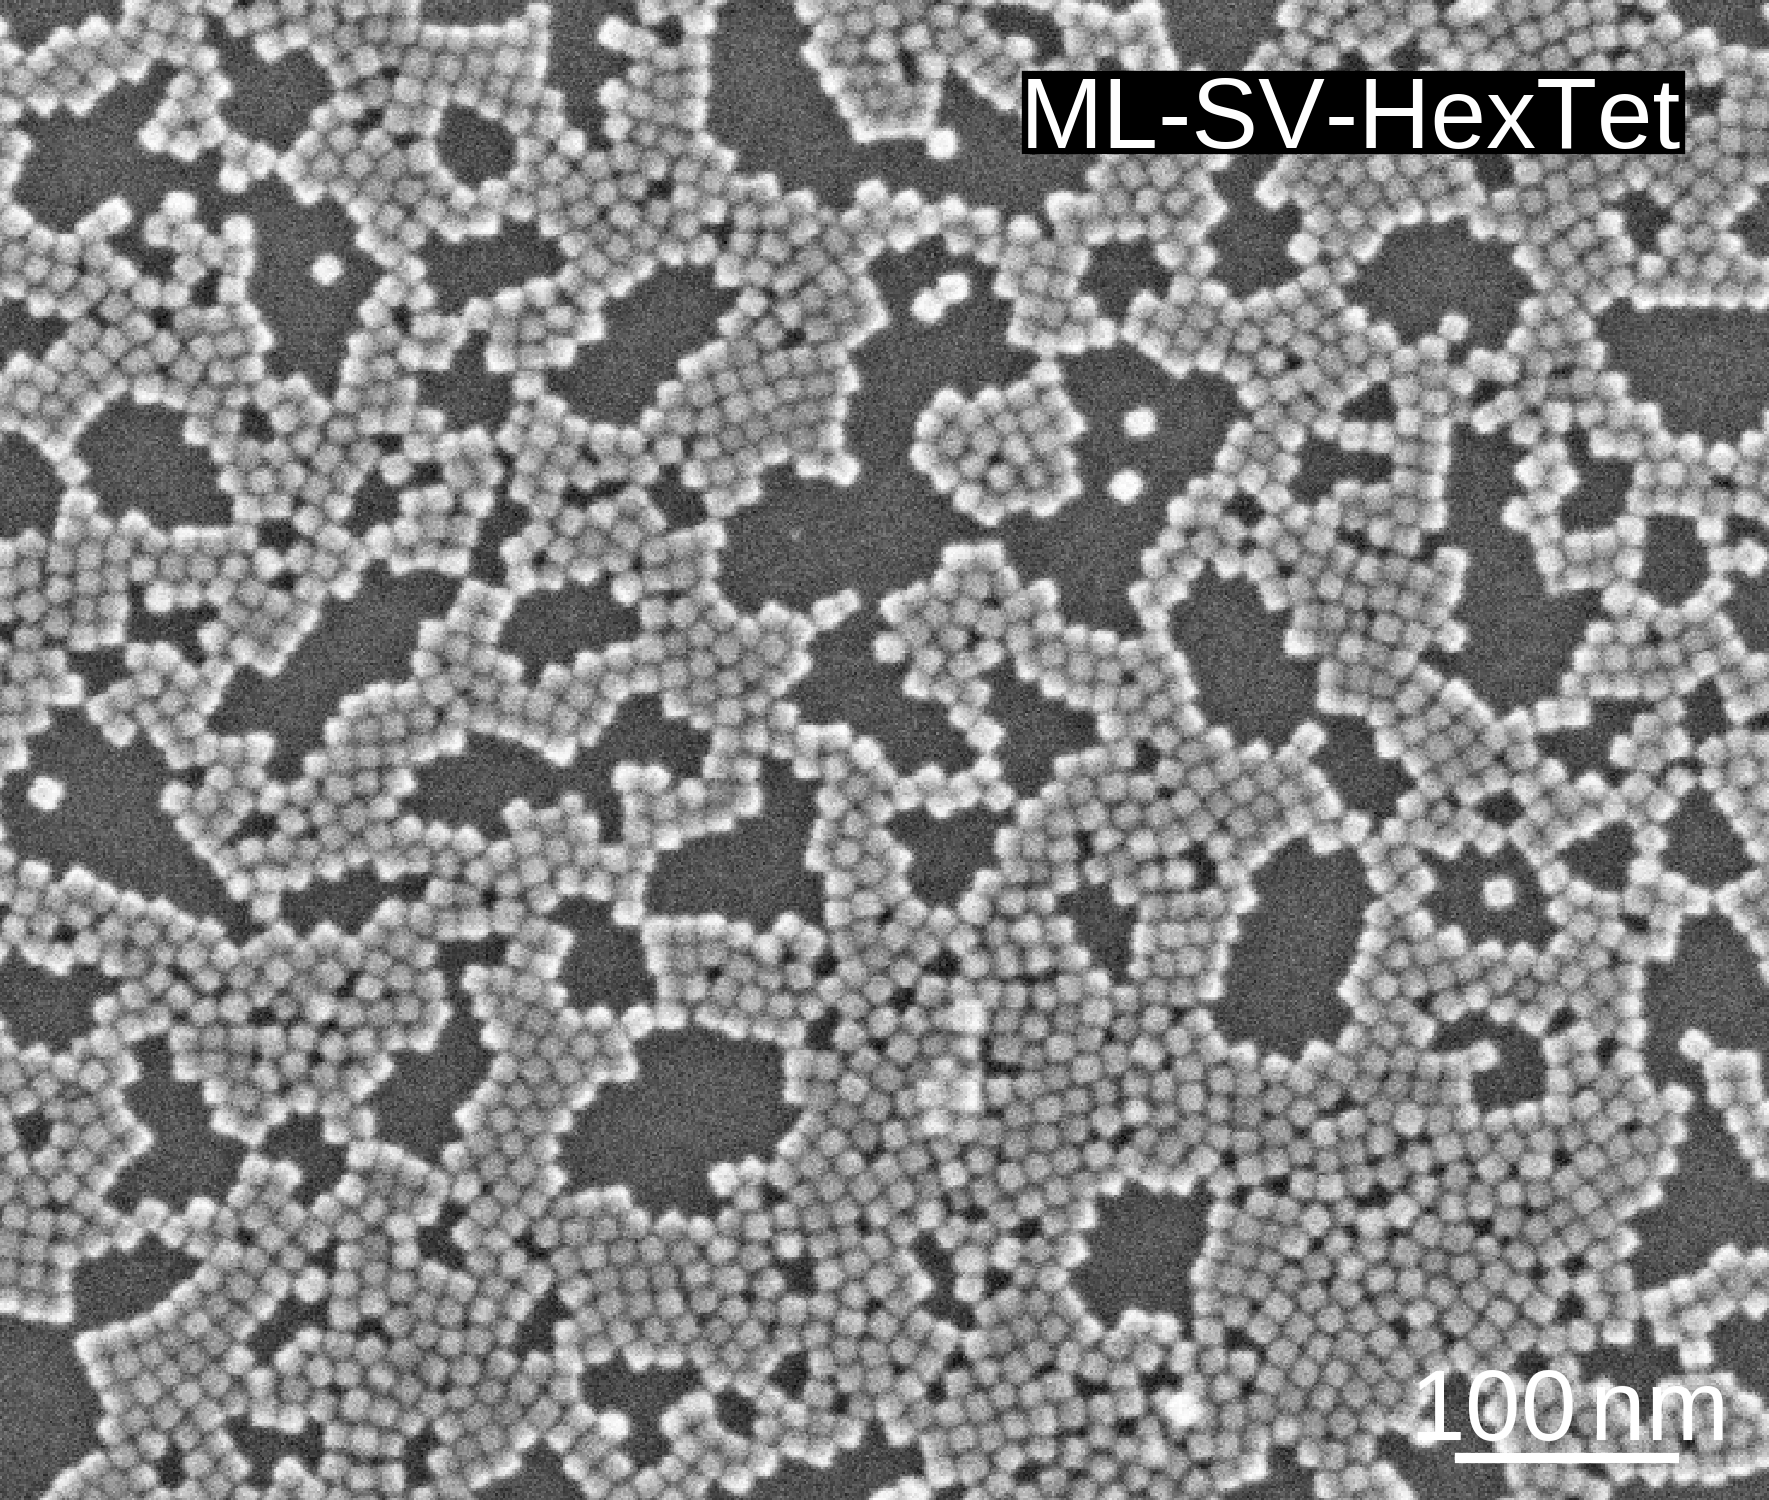
\includegraphics{monolayers_SEM_ML-SV-HexTet}
    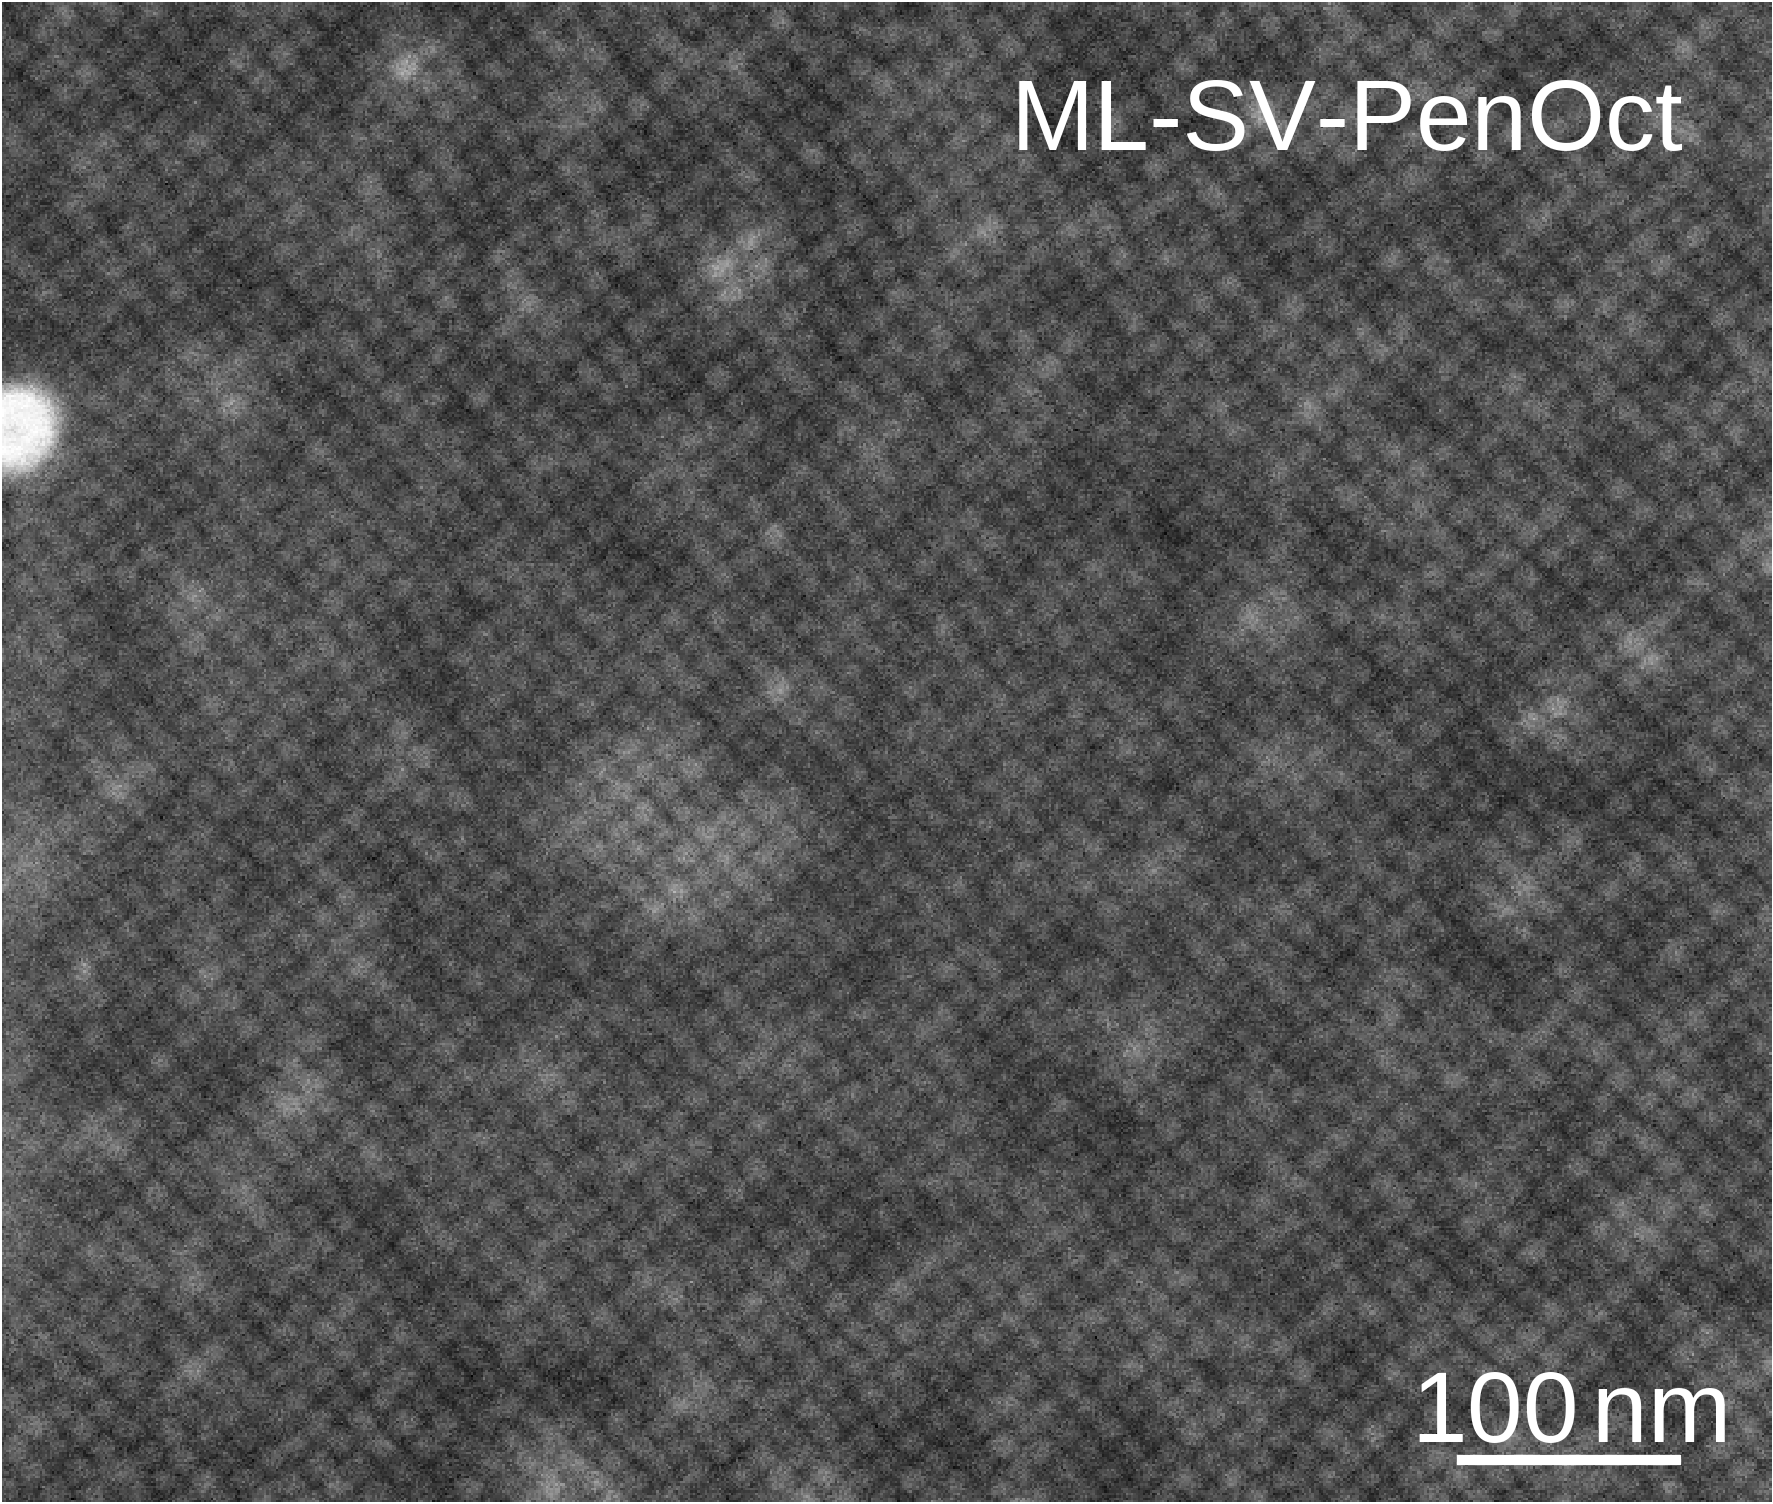
\includegraphics{monolayers_SEM_ML-SV-PenOct}
    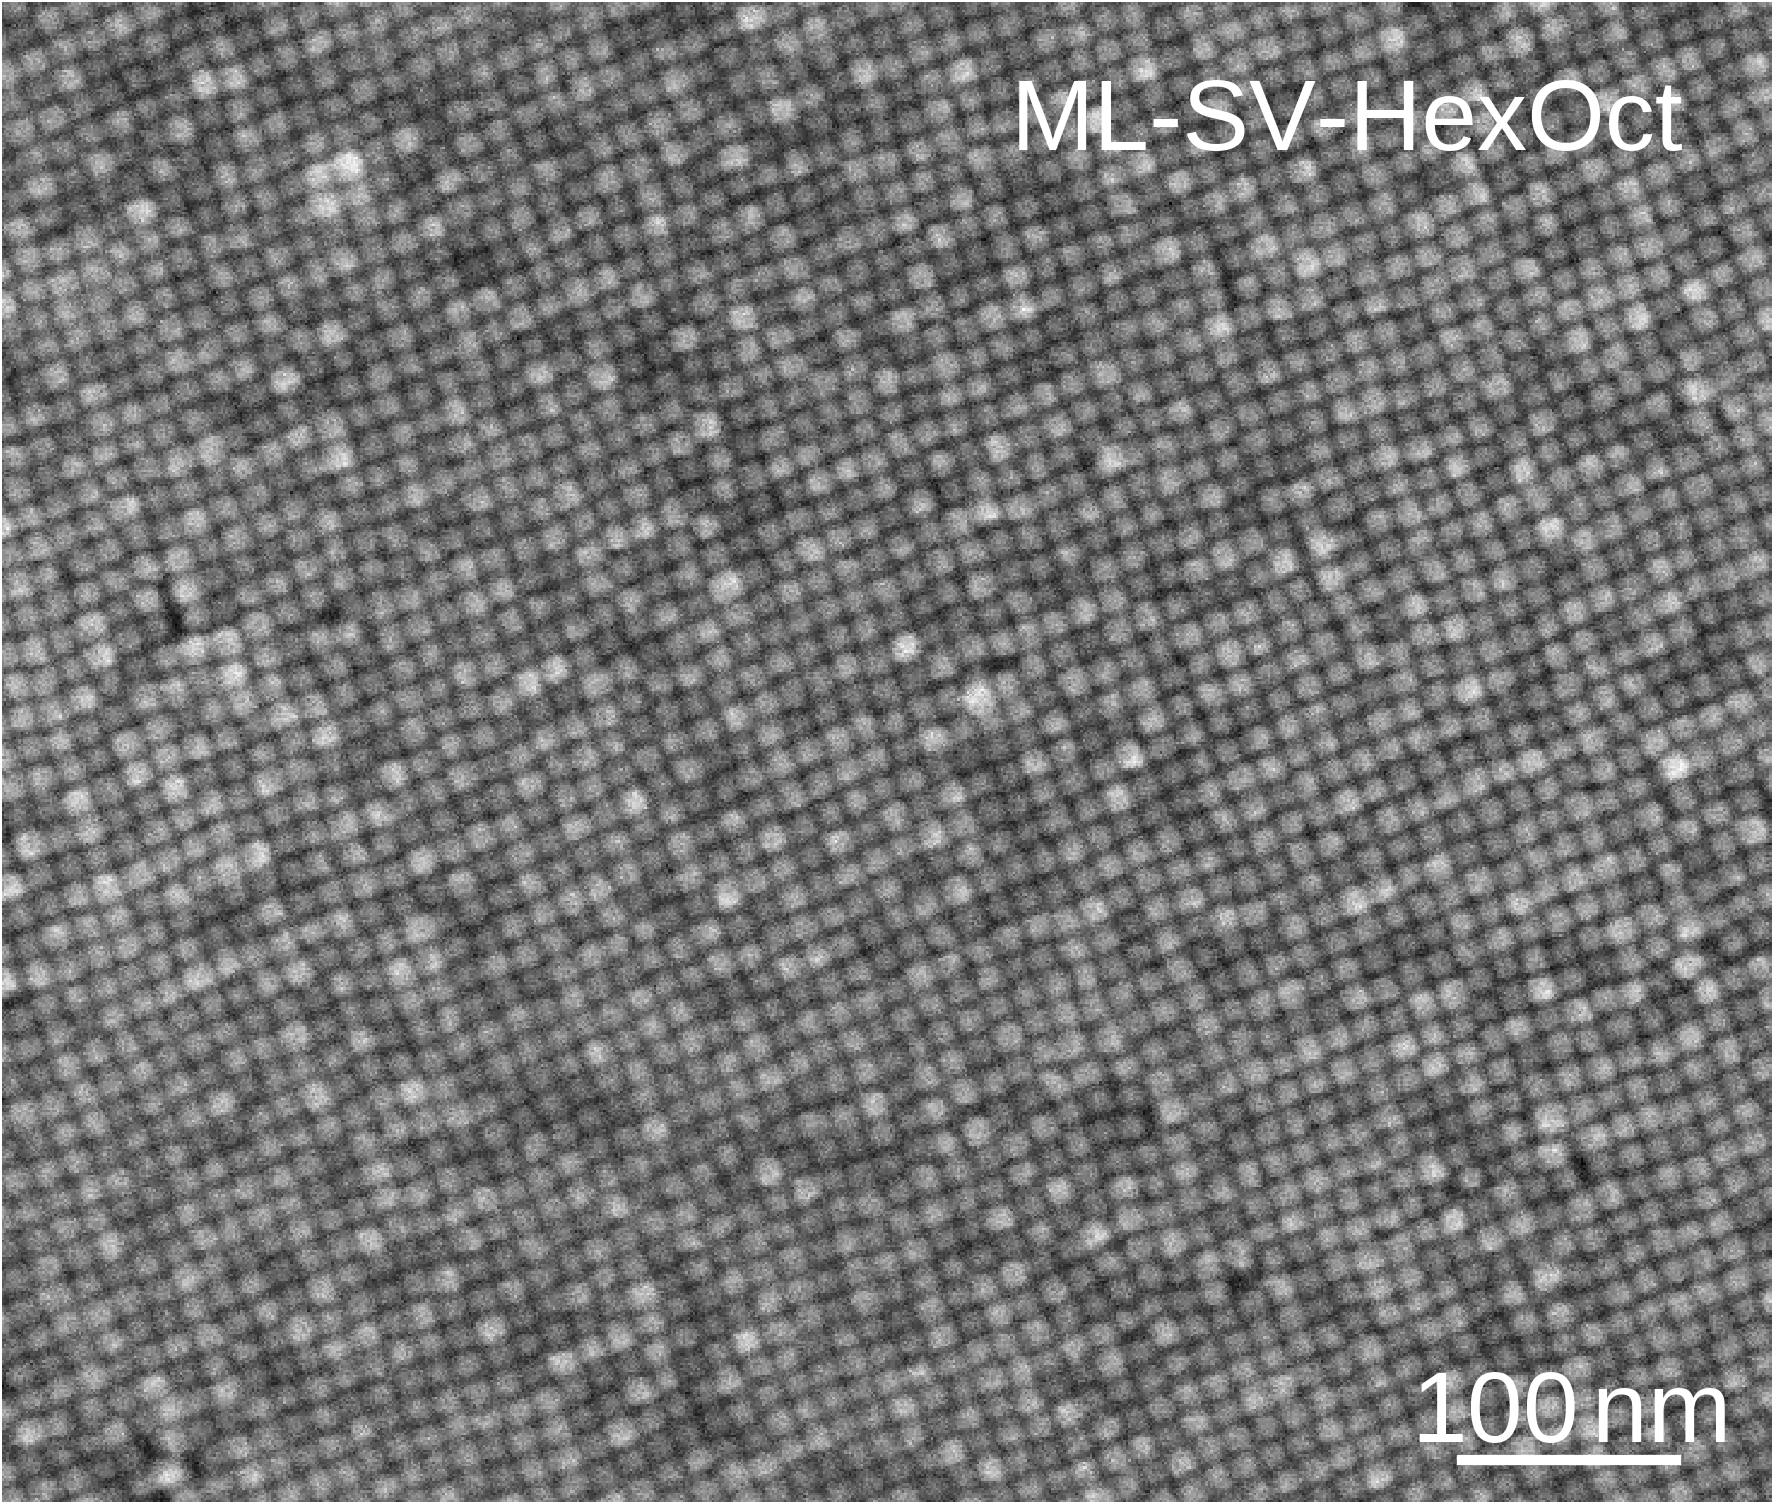
\includegraphics{monolayers_SEM_ML-SV-HexOct}
    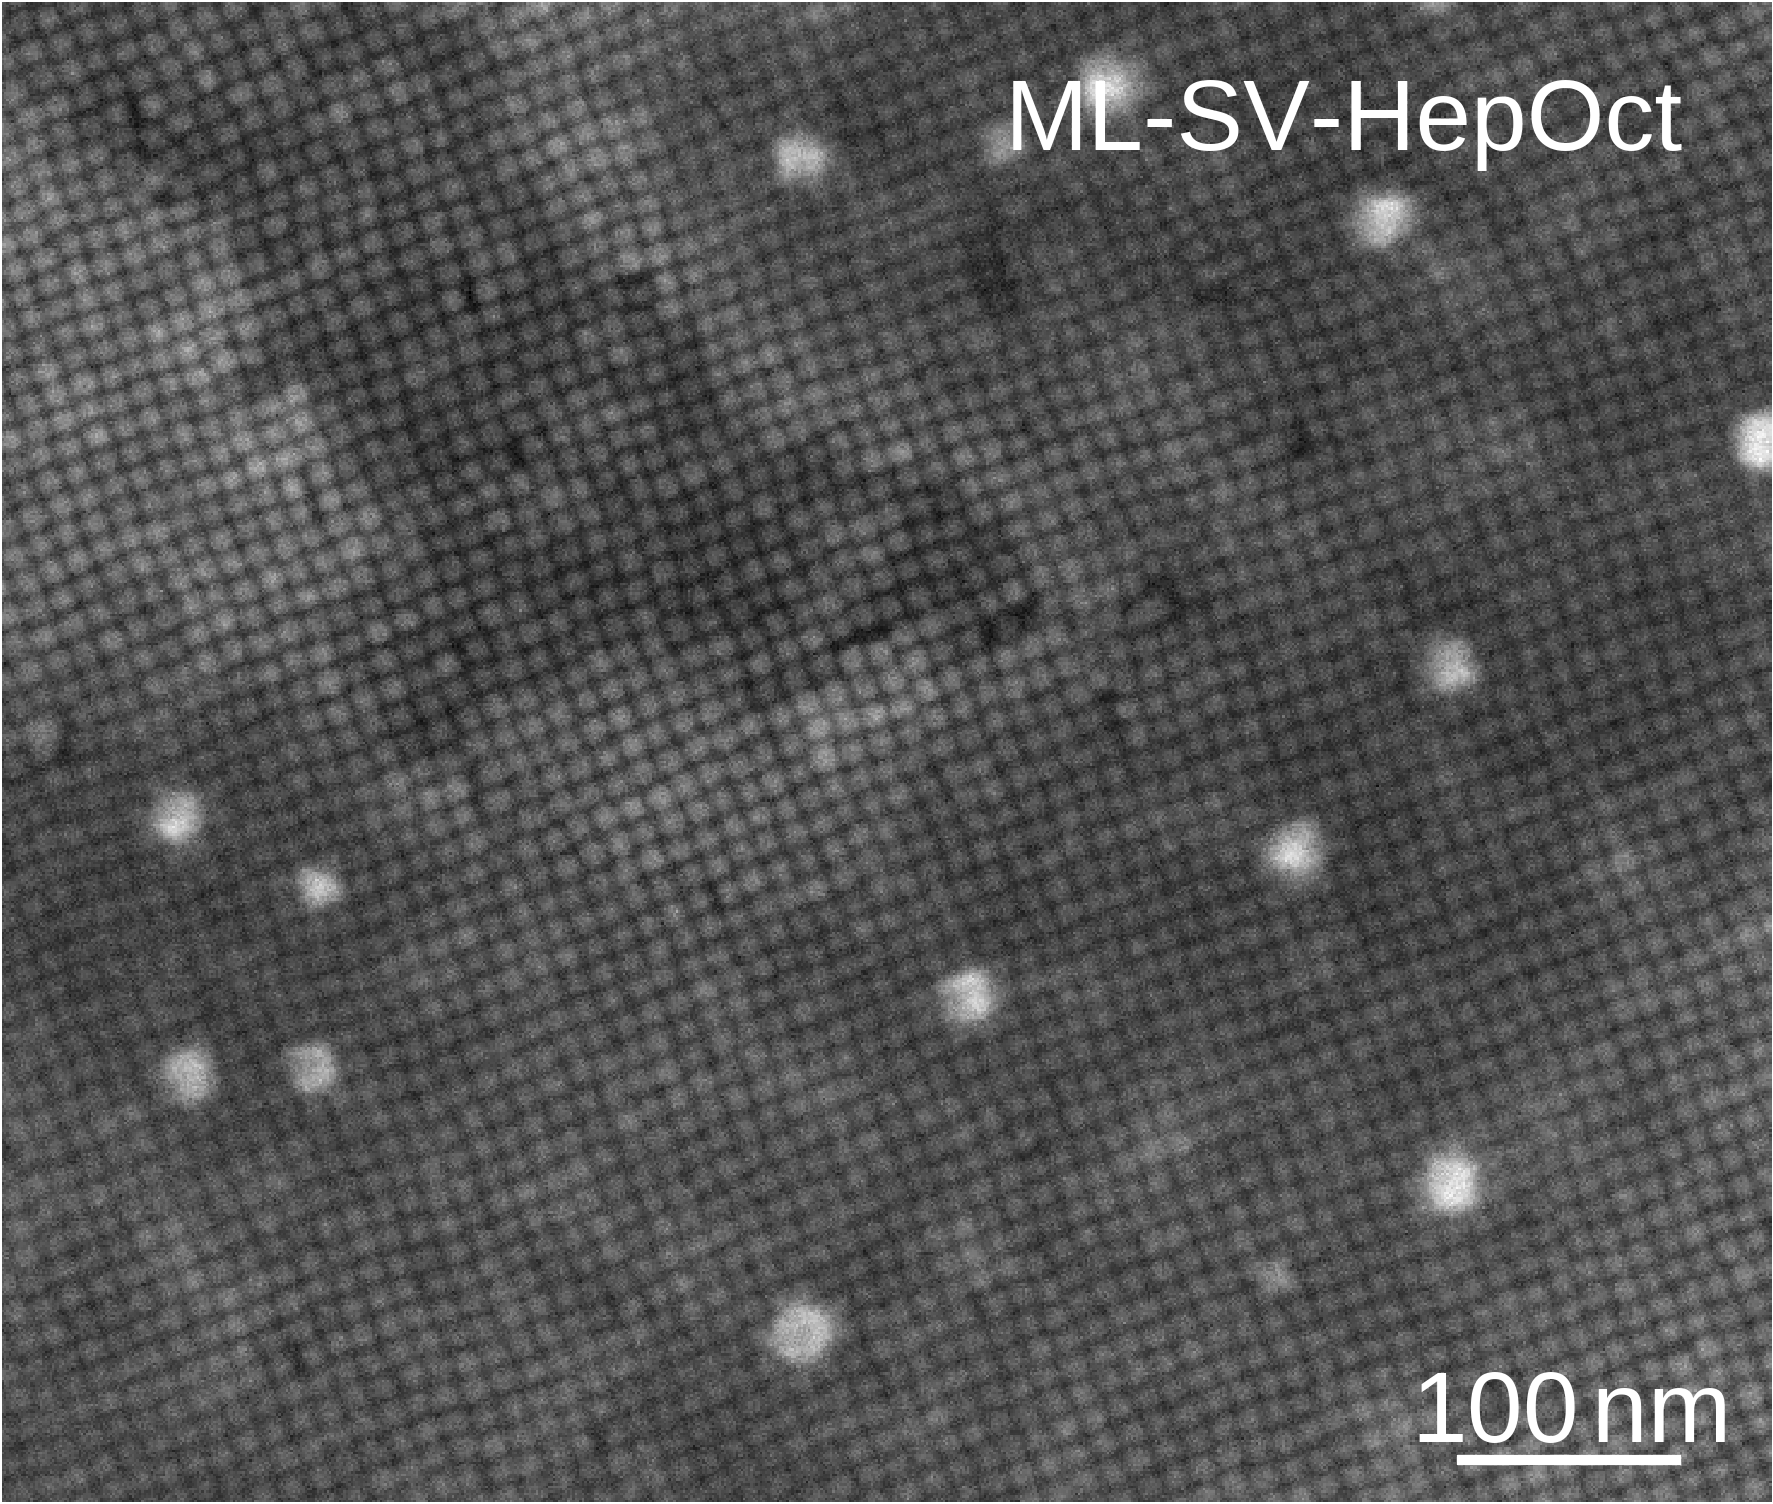
\includegraphics{monolayers_SEM_ML-SV-HepOct}
    \caption{\label{fig:monolayers:preparation:solventVariation:sem}Scanning electron microscopy of Ol-CoFe-C nanoparticles after drop casting using hexane/tetradecene (upper left),  pentane/octadecene (upper right), hexane/octadecene (lower left) and heptane/octadecene (lower right) as solvents.}
  \end{figure}

  Scanning electron microscopy is performed (\refapp{app:additionalExperimentalTechniques:sem}) for a first evaluation of the samples and to study the local order.
  In \reffig{fig:monolayers:preparation:solventVariation:sem} four exemplary samples of combinations are shown: A sample to show a combination of a alkene with a relatively low boiling point, 1-tetradecene, with n-hexane (ML-SV-HexTet), and three samples to show combinations of 1-octadecene with the varied alkanes n-pentane (ML-SV-PenOct), n-hexane (ML-SV-HexOct) and n-heptane (ML-SV-HepOct).
  ..Further combinations are given in App ??..
  A result that is imminently visible from SEM is that an alkene with a relatively low boiling point leads to no order formation. 
  Combinations with 1-octadecene however show for all alkanes local square order formation.
  For the variation of the alkane component, the local evaluation of SEM images shows only minor qualitative differences.

  \begin{figure}[tb]
    \centering
    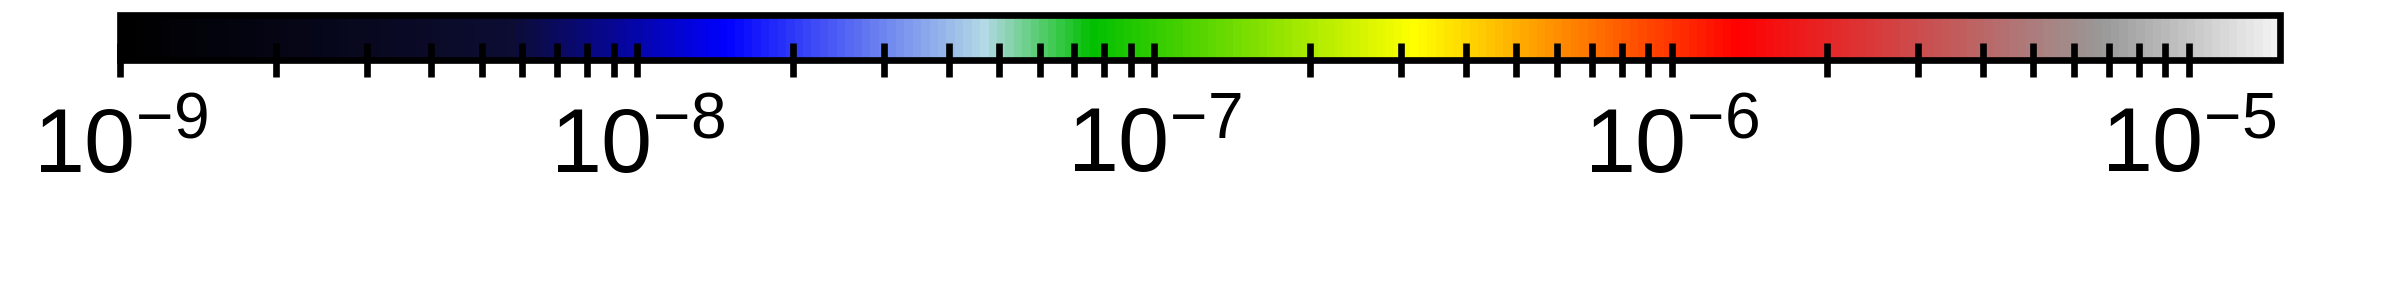
\includegraphics{monolayers_GISAXS_SVcbar}
    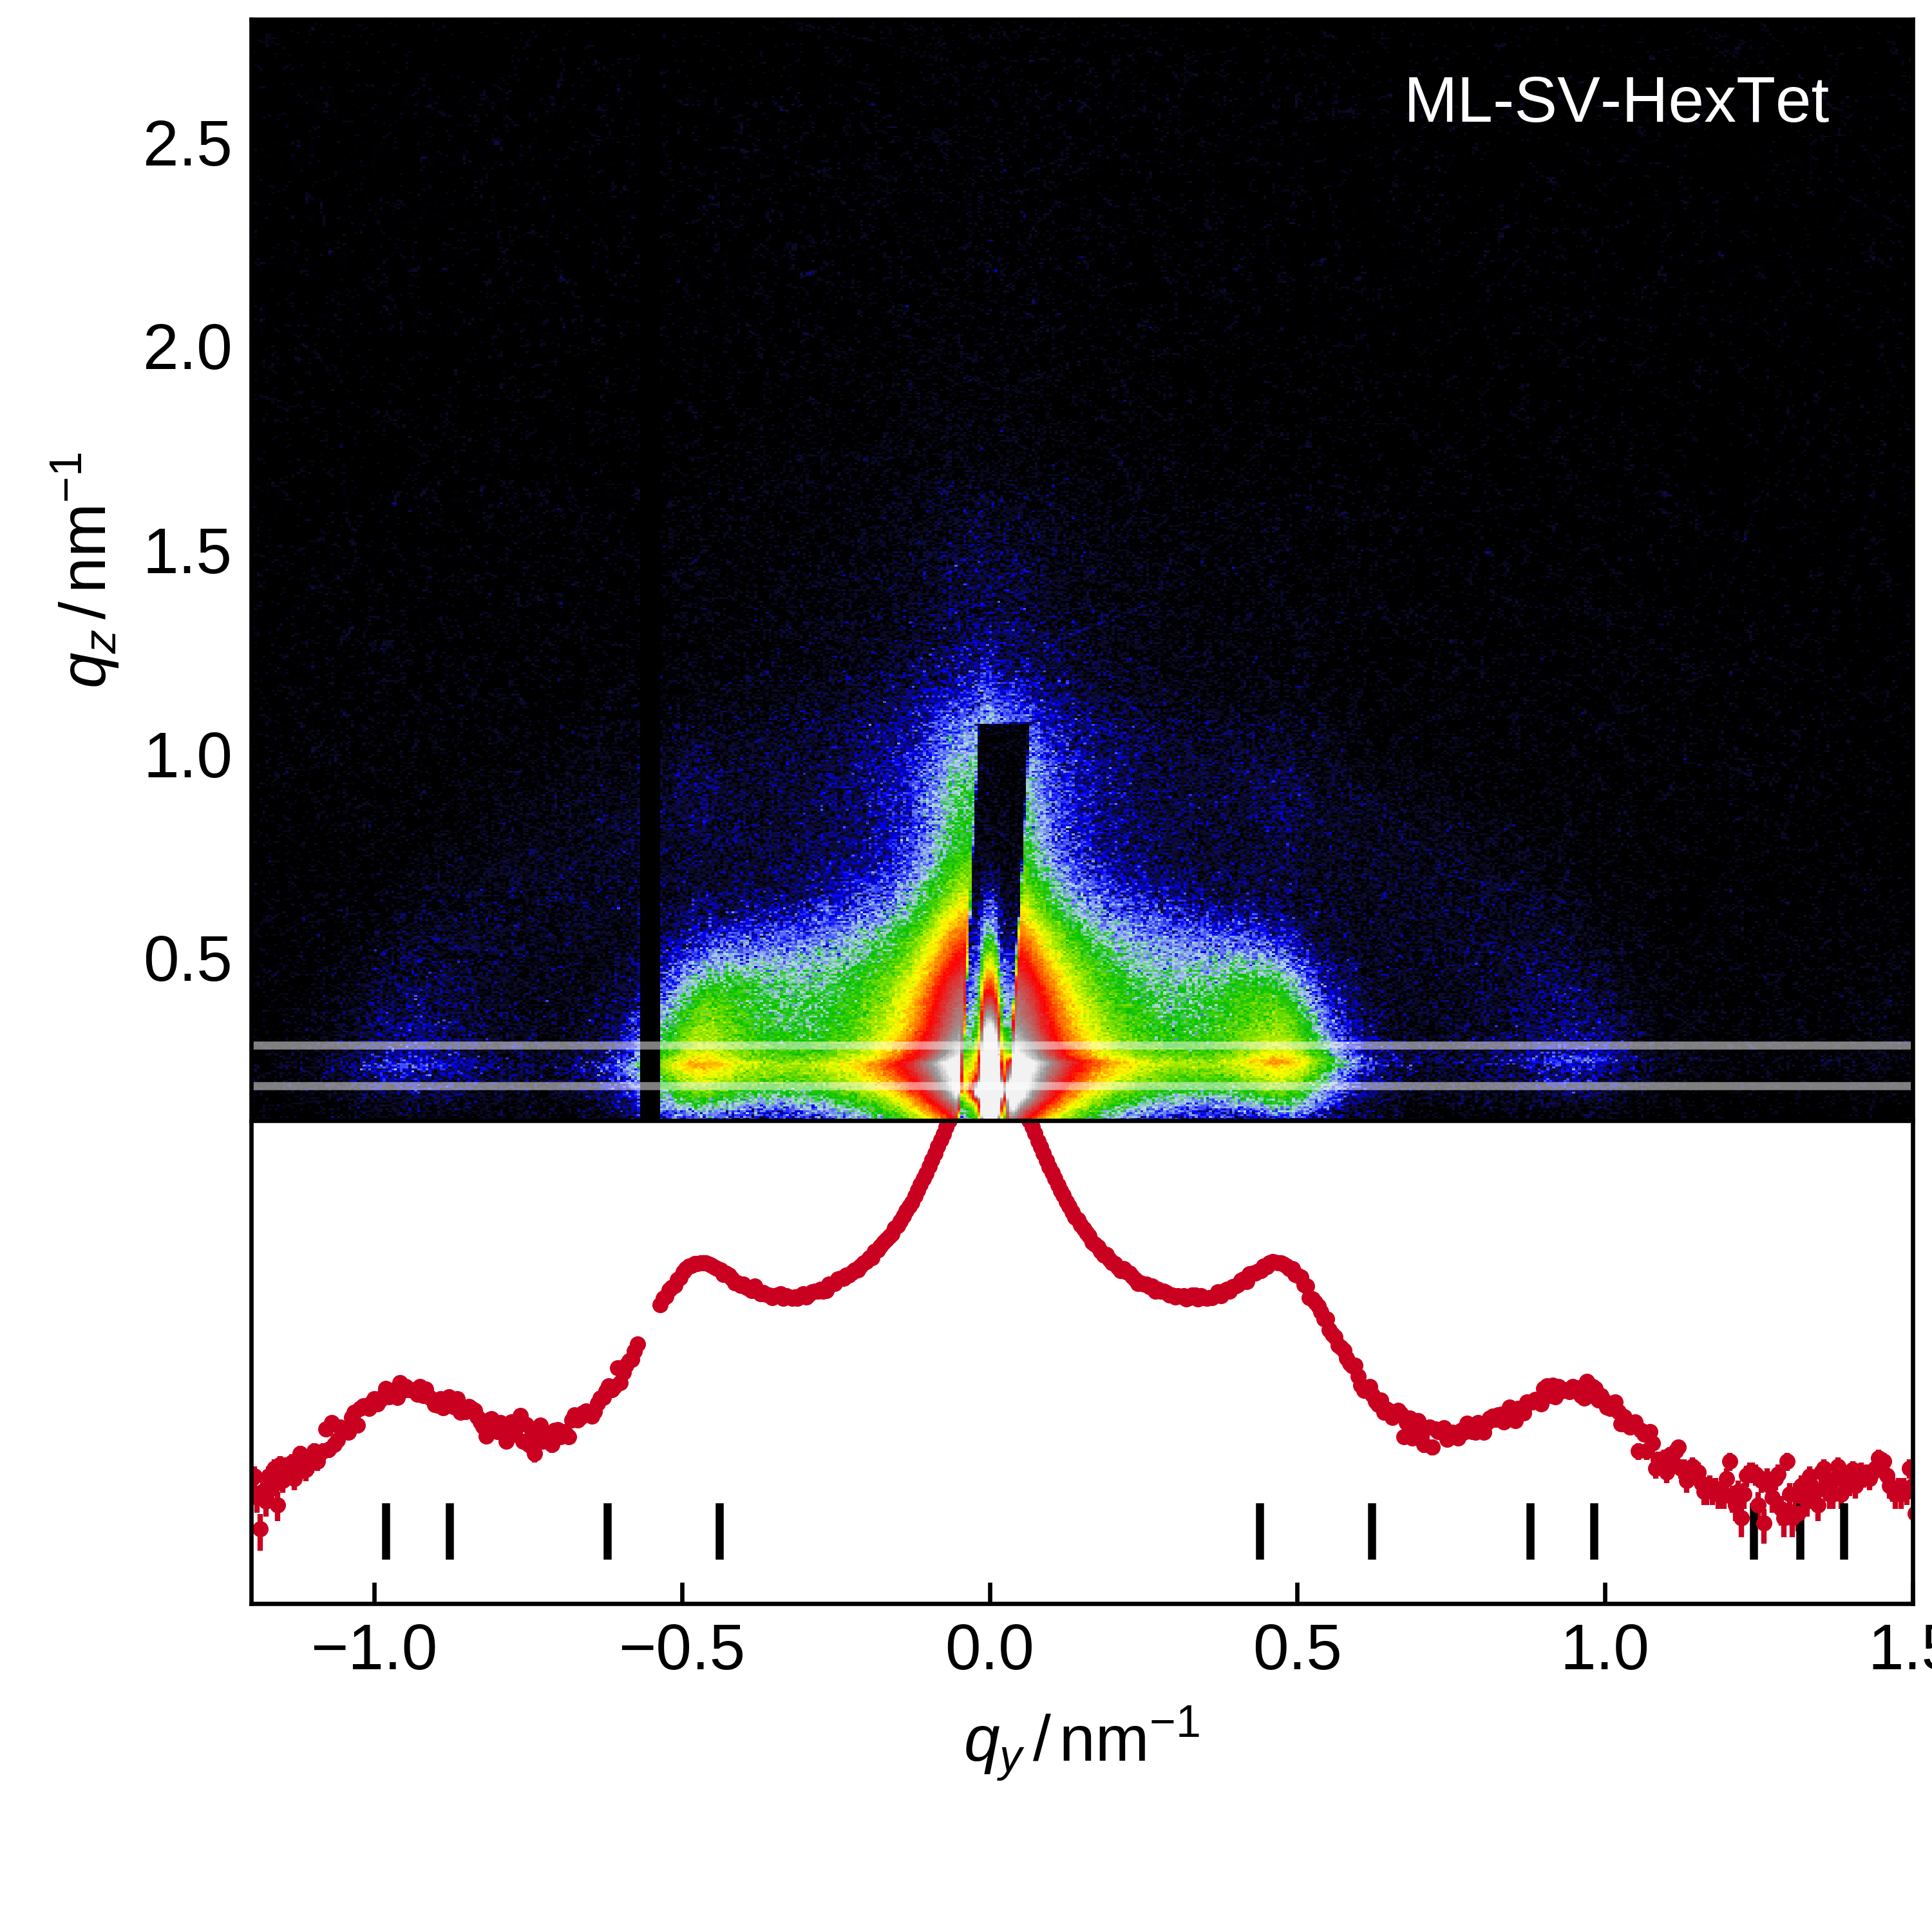
\includegraphics{monolayers_GISAXS_ML-SV-HexTet}
    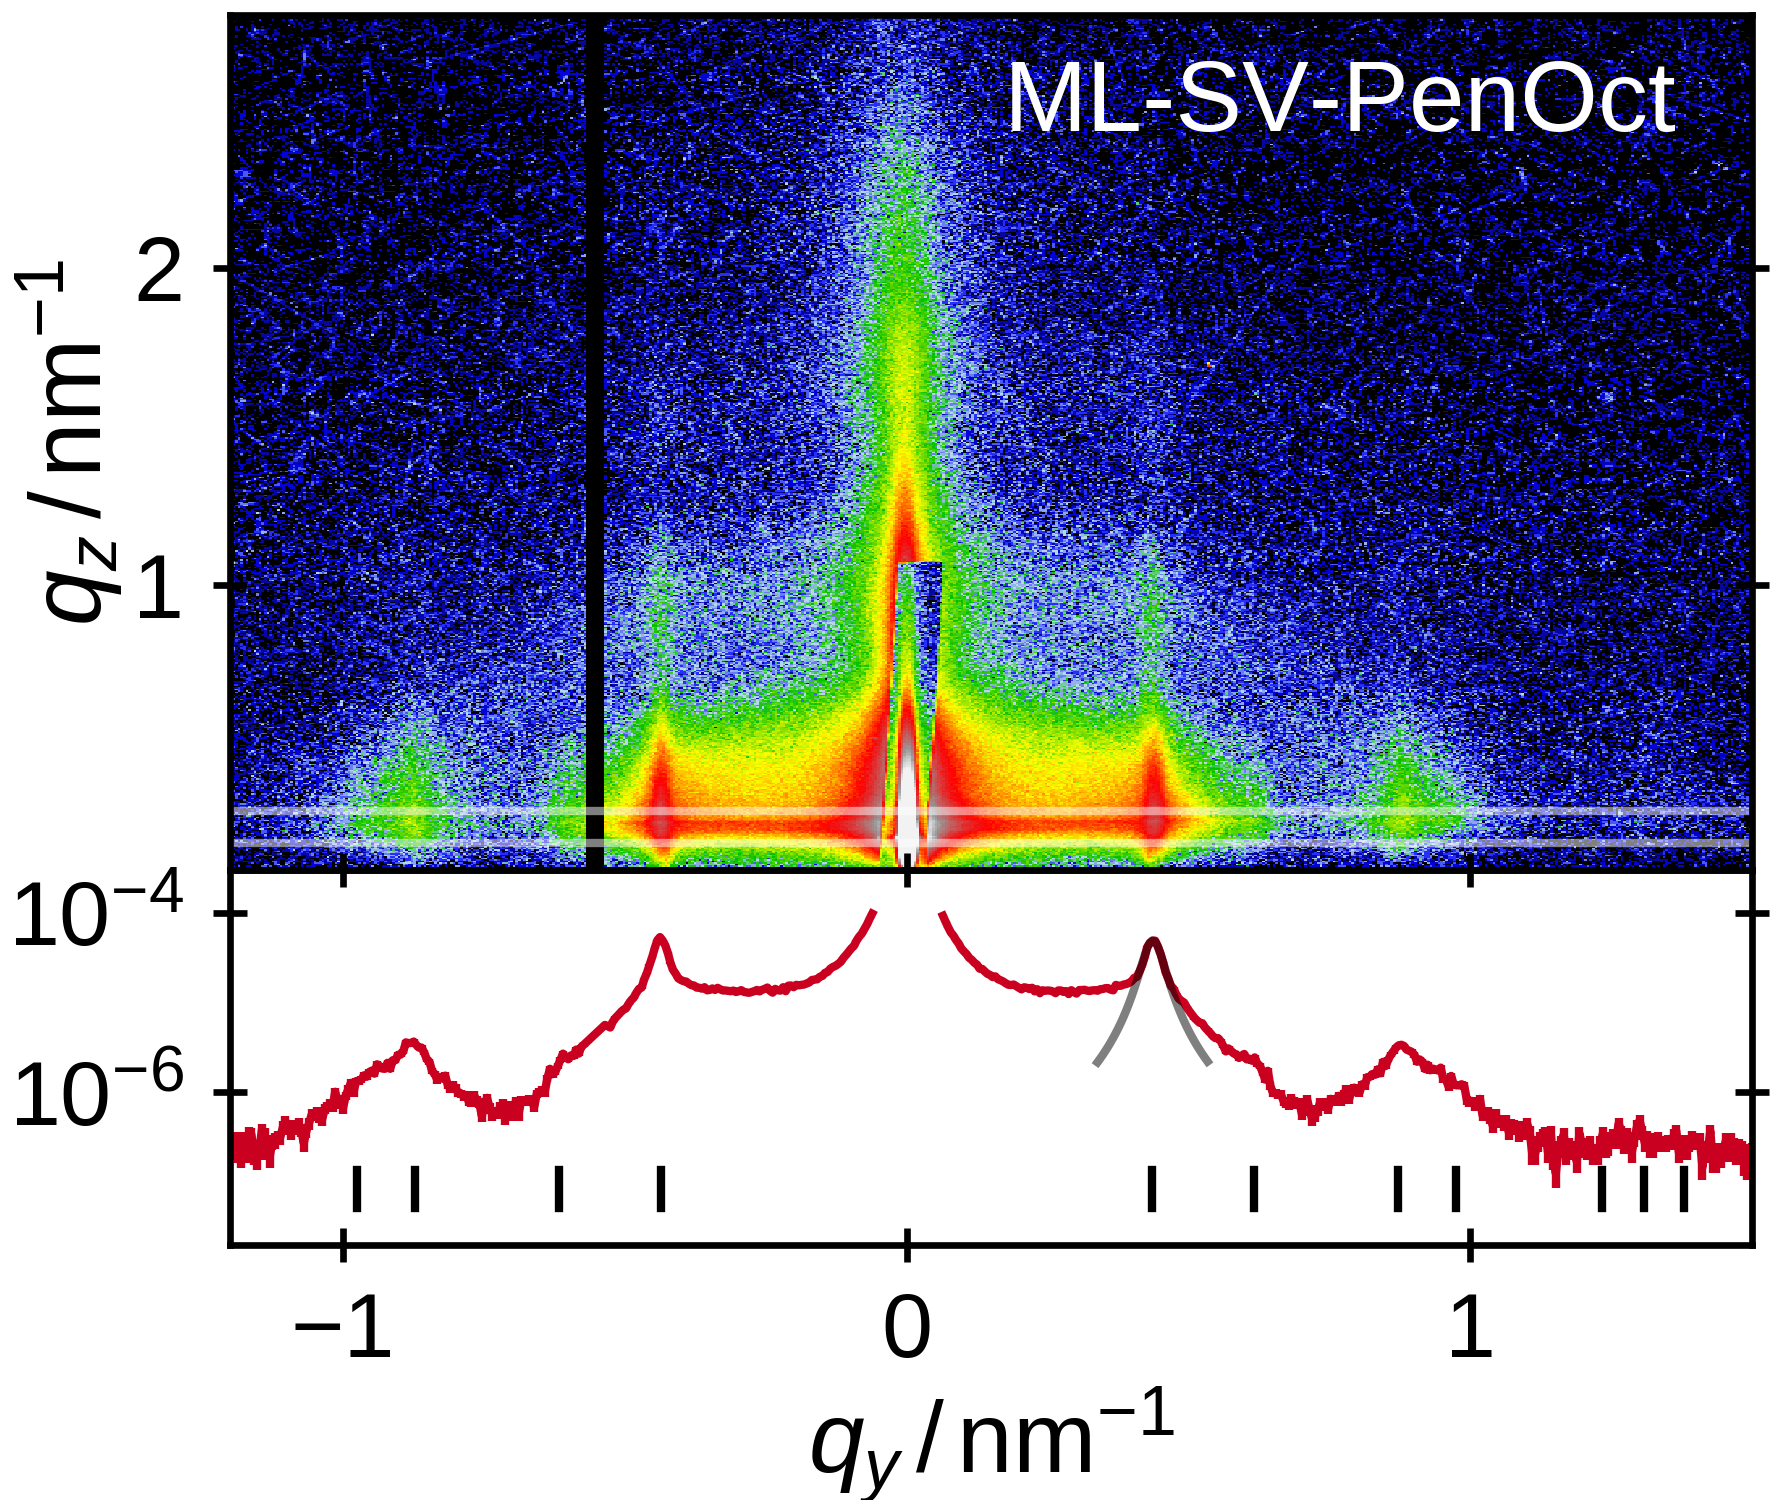
\includegraphics{monolayers_GISAXS_ML-SV-PenOct}
    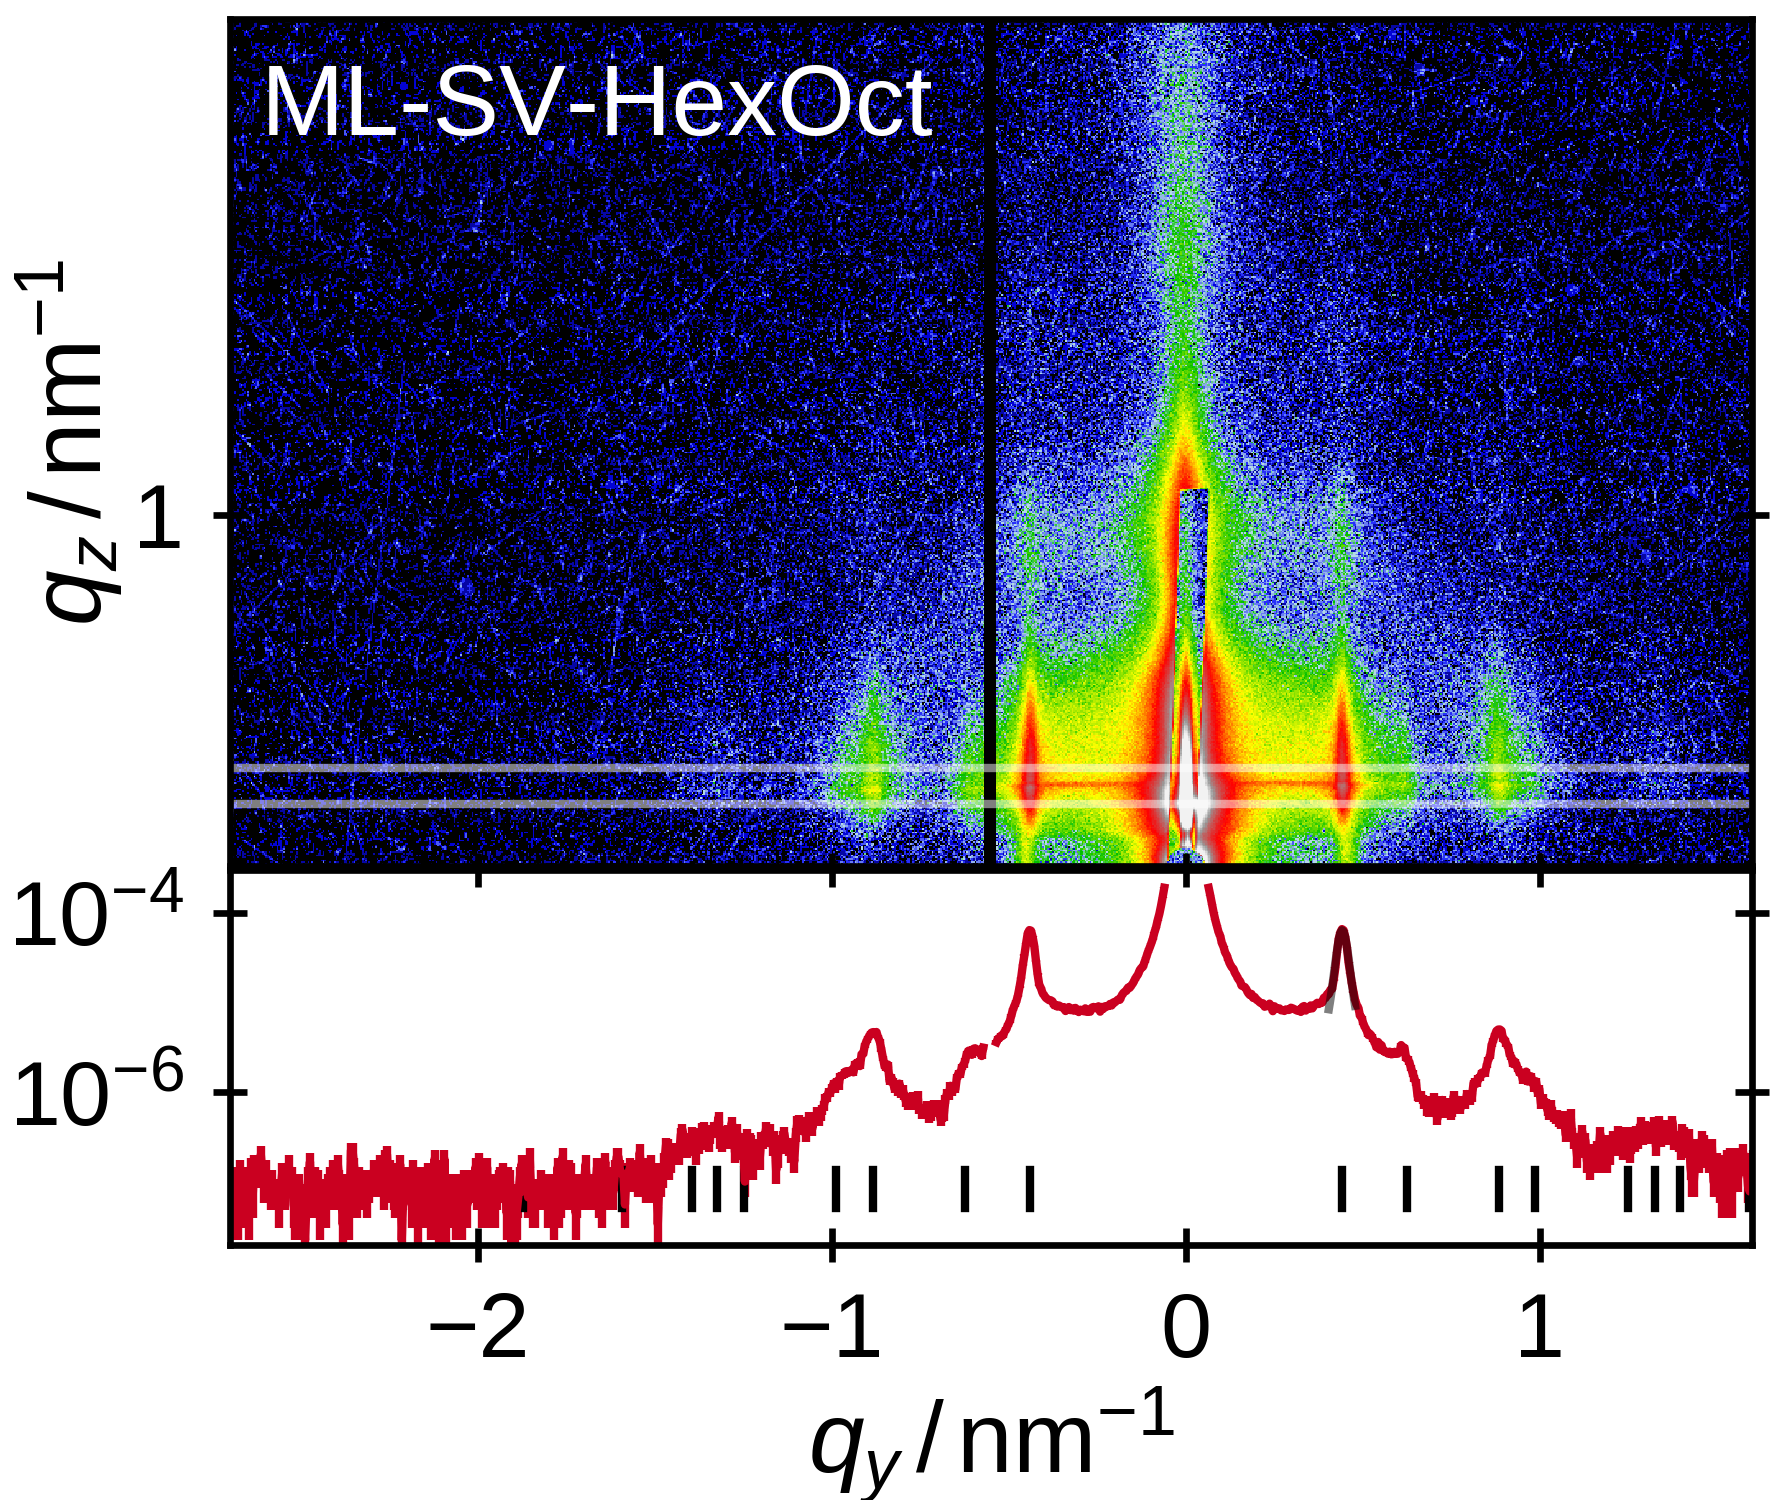
\includegraphics{monolayers_GISAXS_ML-SV-HexOct}
    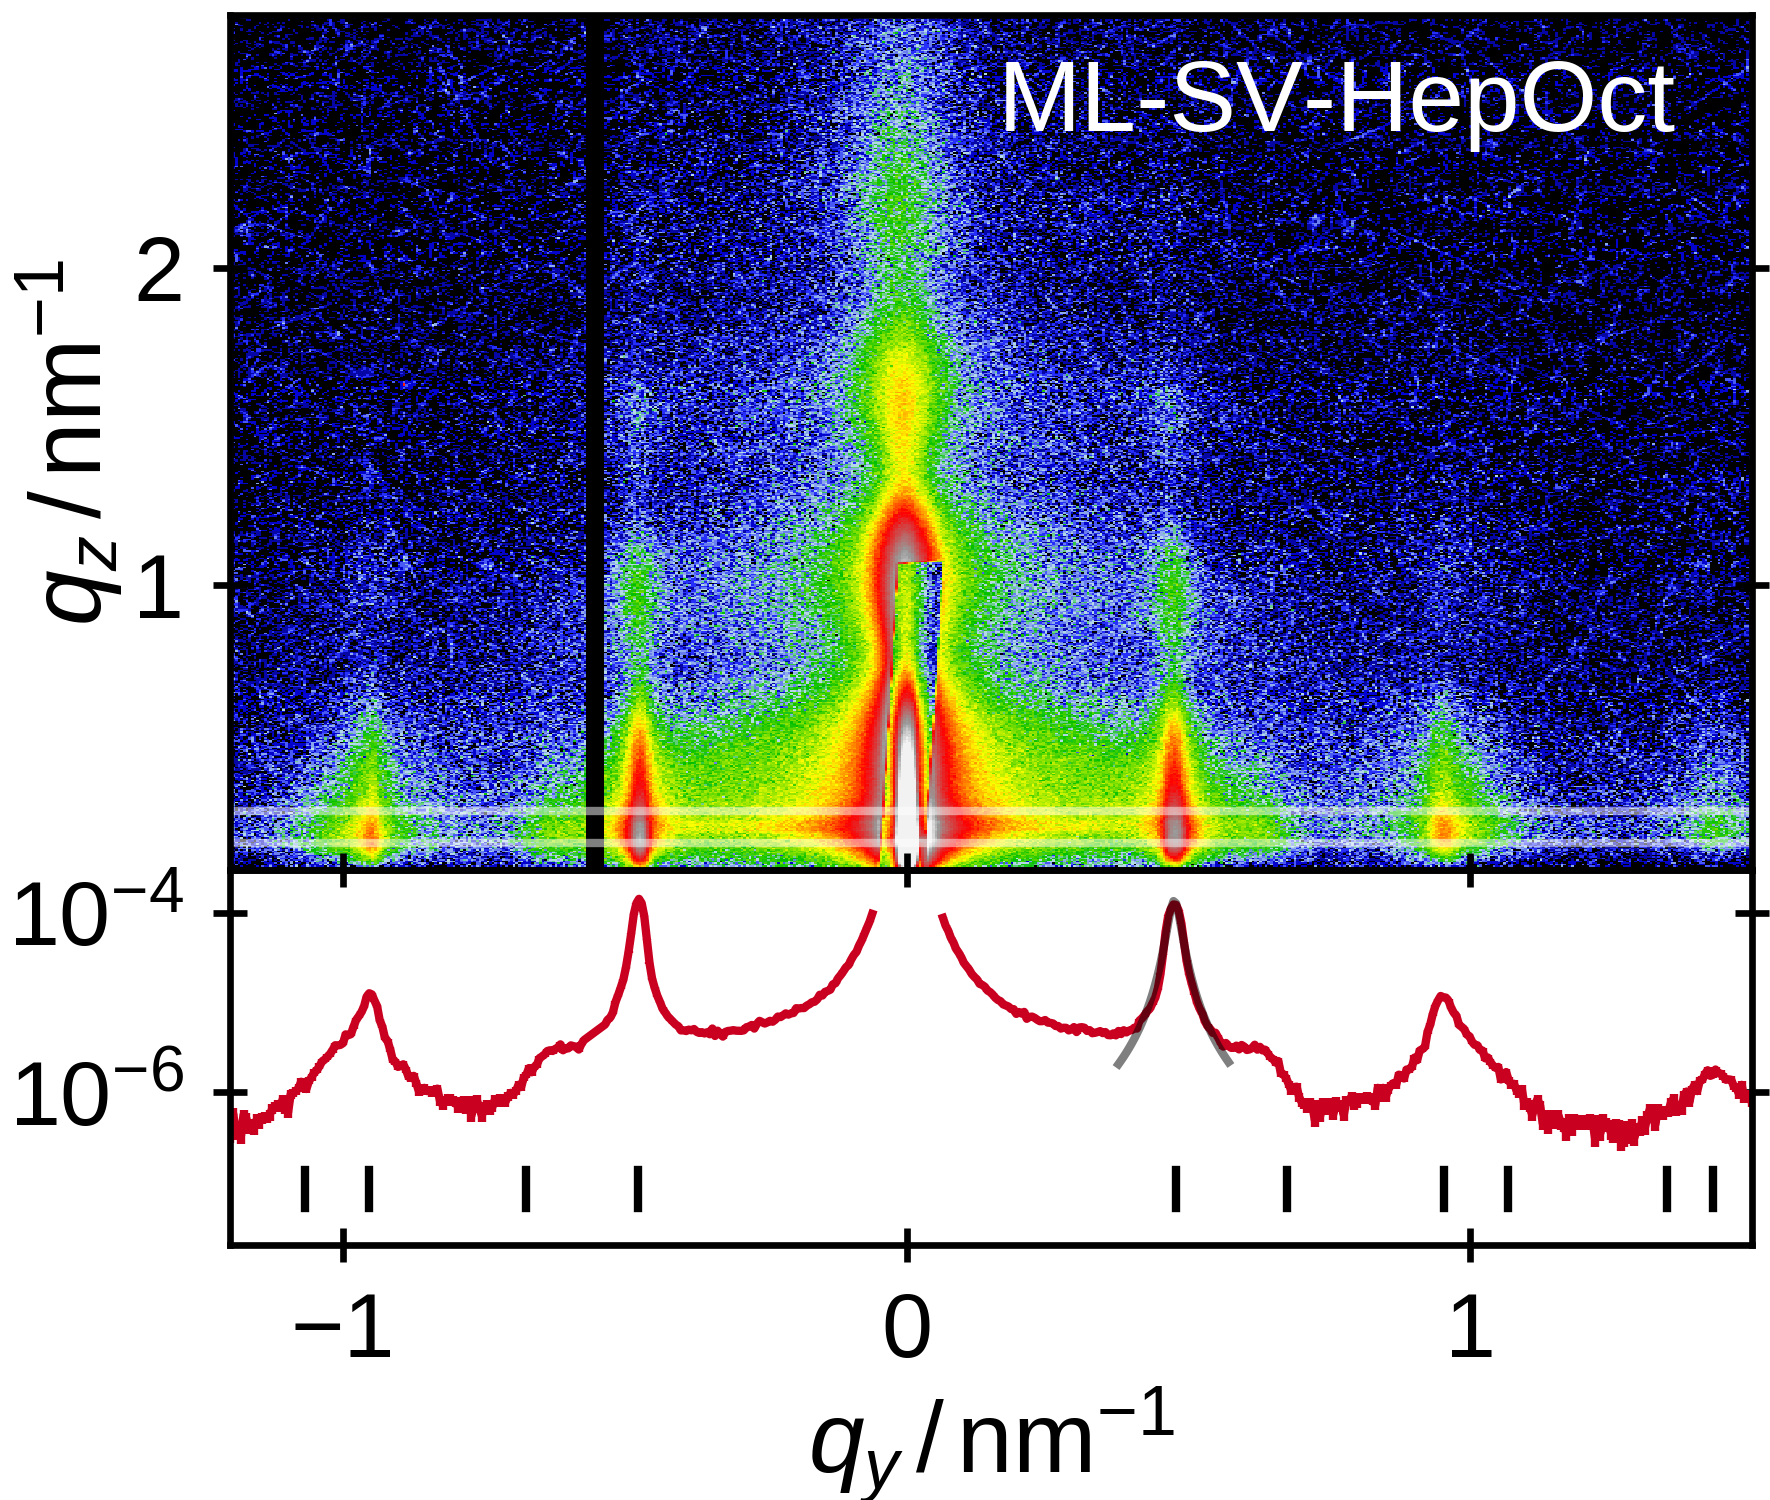
\includegraphics{monolayers_GISAXS_ML-SV-HepOct}
    \caption{\label{fig:monolayers:preparation:solventVariation:gisaxs}GISAXS detector images to study the average lateral structure globally for the same samples as shown in \reffig{fig:monolayers:preparation:solventVariation:sem}. Below the detector images, the scattered intensity in a strip around the Yoneda line. For the ordered samples, the first order peak is fitted to a Lorentzian function with the parameters tabulated in \reftab{tab:monolayers:solventProperties:GisaxsLatticeParams}.}
  \end{figure}
  Thus to quantify the in-plane order, the selected samples are measured using grazing incidence small-angle x-ray scattering at GALAXI (\refapp{ch:appendix:lss:galaxi}) under an incident angle of $\alpha_i \eq 0.11 \unit{^\circ}$.
  The resulting detector images are shown in \reffig{fig:monolayers:preparation:solventVariation:gisaxs}.
  Similar to SEM, ML-SV-HexTet shows no significant structure factor along the Yoneda line, but mainly scattering coming from the form factor of the individual nanoparticles.
  For the other three shown samples, higher order alkanes show the emergence of structure peaks, where the relative intensity of the first order peak increases with the order of the alkane.

  The peak positions are compared to the expected relative positions for a square lattice, given by
  \begin{align}
    q_{hk} \eq \frac{2 \pi}{a} \sqrt{h^2 + k^2},
  \end{align}
  where $h$, $k$ are integers and $a$ the lattice constant of the square arrangement, which is estimated from the (10) peak position.
  For ML-SV-HexOct the position of all peaks fits to this pattern, whereas for ML-SV-PenOct and ML-SV-HepOct the (11) peak position is less visible.
  This effect can be attributed to the unlucky coincidence that the (11) peak position is within the formfactor minima in these cases.

  \begin{table}[tb]
    \centering
    \caption{\label{tab:monolayers:solventProperties:GisaxsLatticeParams}Position and width of the first order peak observed in the GISAXS detector images in \reffig{fig:monolayers:preparation:solventVariation:gisaxs}.}
    \begin{tabular}{ c || l | l || l | l }
      Sample  & $q_{10}$ / $\unit{nm^{-1}}$ & $\Delta q_{10}$ / $nm^{-1}$ & $a$ / nm & $d_{coh.}$ / nm \\
      \hline
      ML-SV-PenOct
        & $0.4367(3)$
        & $0.0210(5)$
        & $14.39(1)$
        & $326(10)$\\
      ML-SV-HexOct
        & $0.43417(3)$
        & $0.0151(4)$
        & $14.22(1)$
        & $503(20)$\\
      ML-SV-HepOct
        & $0.4747(6)$
        & $0.0122(8)$
        & $13.24(2)$
        & $705(85)$\\
      \hline
    \end{tabular}
  \end{table}

  In \reftab{tab:monolayers:solventProperties:GisaxsLatticeParams}, the position and width of the first order peak for the three different samples prepared with 1-octadecene is listed.
  The inverse width of the structure factor peaks is a direct measure of the coherence length of the lattice \cite{Renaud_2009_Probi}.
  Therefore GISAXS provides here a direct measure of the lattice constant and the coherence length of the square lattice.
  The parameters are estimated by fitting a Lorentzian function
  \begin{align}
    I(q_y) \eq \frac{A} {((q_y - q_{10})/\Delta q_{10})^2 + 1},
  \end{align}
  to the intensity around the (10) peak.
  The lattice constant and coherence length is then obtained by
  \begin{align}
    a &\eq \frac{2 \pi}{q_{10}}, \\
    d_{coh.} &\eq \frac{2 \pi}{\sqrt{ \Delta q_{10}^2 - \Delta q_{D.B.}^2 }},
  \end{align}
  with $\Delta q_{D.B.} \eq 0.0083(3) \unit{nm^{-1}}$ the width of the direct beam, which is shown in \reffig{fig:appendix:lss:galaxi:directBeam}.

  The table shows that for increasing order of alkane, the lattice constant reduces and the coherence length increases.
  Both can be explained by an improved packing of the square lattice and therefore this is in agreement with the qualitative observation that higher alkanes increase the sample quality.
  A further qualitative assessment of a combination from n-octane/1-octadecene shows that the sample quality decreases again at this point.
  As well as that the combination n-heptane/1-hexadecene is of lower quality, whereas the combination of higher order alkenes is not feasible at ambient conditions, as here the freezing point of the alkenes is above room temperature.

  In summary, the best quality of samples from a series of alkane/alkene combinations is achieved for a combination of n-heptane together with small addends of 1-octadecene.
  An approach to an explanation of this specific combination can be given in the freezing point of 1-octadecene and the evaporative cooling properties of n-heptane.
  1-octadecene freezes at a temperature of approx. $15 \unit{^\circ C}$, whereas evaporating n-heptane can cool a surface by $\Delta T \eq 8 \unit{^\circ C}$.
  Thus, it can be assumed that during evaporation of the quickly evaporating n-heptane, the surface of the droplet is cooled near the freezing temperature of 1-octadecene, which increases the viscosity of the liquid at the surface.
  This generates the condition needed for a monolayer formation as described in \cite{Bigioni_2006_Kinet}, where particles are pinned to the surface of the evaporating droplet at which they can find one another to form a single ordered layer.
  Increasing the order of the alkane removes the evaporative cooling component from the drop casting experiment, as to why there is no order observed above n-heptane.
  Decreasing the order of the alkane, increases the evaporative cooling effect, but also decreases the time the particles have to order themselves with great mobility.
  On the other hand, exchanging 1-octadecene for a lower order alkene reduces the freezing point greatly, as to which no order is observed here once again.


  A more detailed investigations of the various combinations
  ...appendix..
  shows that, while combinations with 1-hexadecene still give rise to some short range order, only combinations with 1-octadecene lead to long range order across several micrometers.


\end{document}